\documentclass[a4paper]{extarticle}
\usepackage[utf8]{inputenc}
\usepackage{hyperref}
\usepackage{geometry}
\usepackage{fancyhdr}
\usepackage{graphicx} % libreria per le immagini
\usepackage{amssymb} %libreria per i simboli (ex. alfabeto reco)
\usepackage{algorithm2e} %libreria per scrivere pseudocodice
\usepackage{longtable}
\usepackage{caption}
\usepackage{lastpage}

\setlength{\parindent}{0em}%indentazione paragrafo
\setlength{\parskip}{1em}%spazio tra paragrafi
\renewcommand{\baselinestretch}{1.3}%interlinea
\graphicspath{ {./} }
\geometry{
    a4paper,
    left=10mm,
    right=10mm,
    bottom=20mm
}


\hypersetup{
    colorlinks=true,
    linkcolor=blue,
    filecolor=blue,      
    urlcolor=blue,
    pdftitle={Overleaf Example},
    pdfpagemode=FullScreen
}

\pagestyle{fancy}
\fancyhf{}
\rhead{Federico Calò}
\lhead{Ingegneria della conoscenza}
\cfoot{  \thepage }


\title{Ingegneria della conoscenza}
\author{\href{http://www.federicocalo.it}{Federico Calò} }
\date{}

\begin{document}
\maketitle
\newpage
\tableofcontents
\voffset -30pt

\newpage

\section*{Intro}

 Il sito a cui si riferisce il professore è Artificial Intelligence: Foundations of Computational Agents, second edition, Cambridge University Press. Del libro vi è presente una versione online presente al seguent \href{https://artint.info/}{link}. Gli appunti sono organizzati in due macro sezioni: gli appunti delle lezioni e gli appunti derivanti dal libro. 

L'obiettivo del corso è quello di acquisire le competenze necessarie alla specifica e progettazione i sistemi intelligenti basati su conoscenza, attraverso la padronanza degli aspetti teorici modelli logico e matematico-statistici e la capacità implementative, di valutazione e miglioramento di sistemi esistenti nei diversi domini applicativi. Inoltre ci si approccerà a problemi complessi mediante modelli di rappresentazione e ragionamento:
 
 \begin{itemize}
 	\item formalismi per la rappresentazione della conoscenza di dominio (proposizionale, multi-relazionale)
 	\item forme i ragionamento automatico
 	\item tecniche di acquisizione della conoscenza (modelli per la predizione) basate sull'apprendimento automatico
 	\item tecniche di valutazione
 	\item modelli di ragionamento/acquisizione in presenza di incertezza: approccio probabilistico esteso anche a rappresentazioni multi-relazionali
 \end{itemize}
 
Per quanto riguarda i capitoli del libro di cui si andrà a prendere spunto per le trattazioni sono:

\begin{itemize}
	\item Introduzione ai sistemi basati su conoscenza [1-2]
	\item Fondamenti - Problemi e Ricerca delle soluzioni [4]
	\item Rappresentazione della conoscenza (Proposizionale) [5]
	\item Rappresentazione di individui e relazioni [13]
	\item Ontologie e BAsi di conoscenza distribuite [14]
	\item Ragionamento in presenza di incertezza [8]
	\item Apprendimento Supervisionato [7]
	\item Apprendimento e incertezza [10]
	\item Modelli probabilistici relazionali [15]
\end{itemize}
 

\newpage 
\section{Lezioni}

\subsection{1 - Introduzione Sistemi basati su conoscenza}

\subsubsection{Introduzione}

Vi sono diverse definizioni dell'ingegneria della conoscenza, una è la seguente:

\begin{center}
	"L'ingegneria della conoscenza (KE) si riferisce a tutti quegli aspetti tecnici, scientifici e sociali che sono coinvolti nella costruzione, mantenimento e uso dei sistemi basati su conoscenza"
\end{center}

Tipicamente l'informazione è definita in termini di dati, conoscenza in termini di informazioni e saggezza in termini di conoscenza. Molto importante è \textbf{la piramide DIKW} (gerarchia della conoscenza)che consiste in una piramide formata da 4 livelli, dal più basso:
\begin{itemize}
	\item Dati (Data)
	\item  Informazioni (Information)
	\item Conoscenza (Knowledge)
	\item Sapere (Winsdom)
\end{itemize}

\begin{figure}[h]
\begin{center}
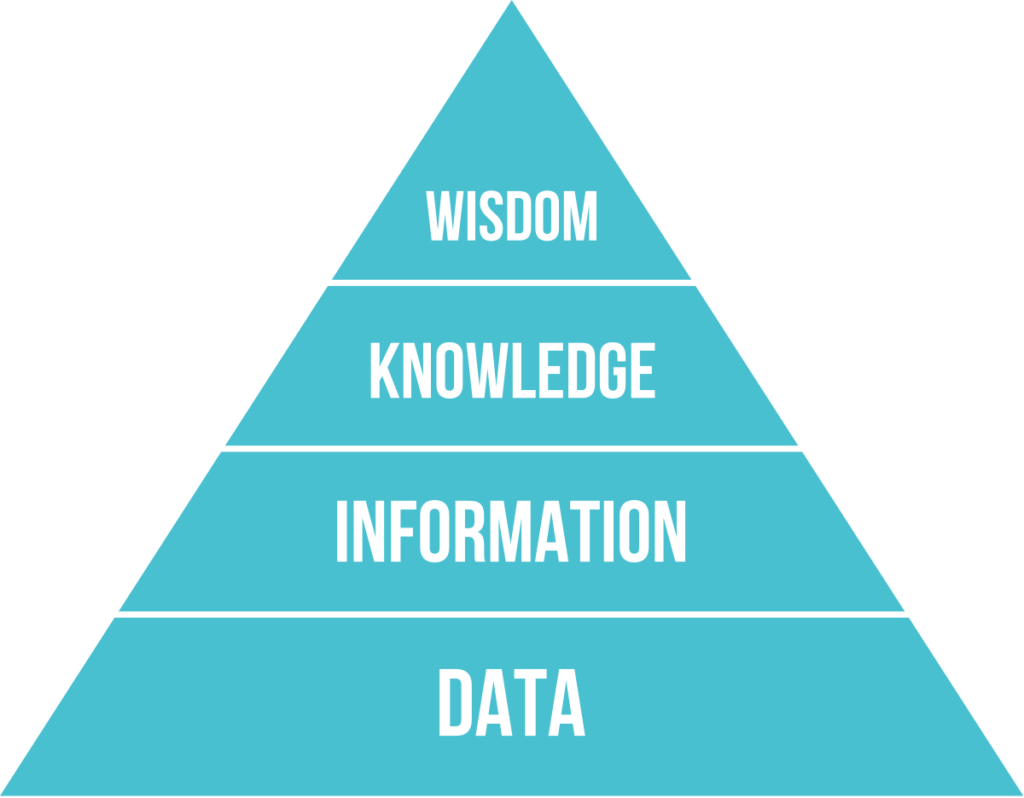
\includegraphics[scale=.3]{wkid.png}
\end{center}

\end{figure}

I \textbf{dati} sono costituiti da segni o simboli che rappresentano simboli o segnali che rimangono inutili fino  quando non sono messi in una qualche forma.  Possono essere \textit{universali} se sono prodotti da osservazioni, oppure \textit{soggettivi} costituite dalle osservazioni stesse. Possono essere costituiti da \textit{fatti}, cioè da osservazioni discrete, oggettive, non organizzate o elaborate che mancano di contesto interpretativo; da \textit{segnali}, cioè da stimoli sensoriali o letture di segnali attraverso sensi o sensori; o \textit{simboli}, cioè da insiemi di segni che rappresentano le percezioni di proprietà di oggetti, eventi dell'ambiente e che vengono registrati al fine della comunicazione.

Le \textbf{informazioni} sono dati dotati di significato e scopo, ottenute per descrizione e distinte dai dati per la oro utilità. Vengono inferite di dati rispondendo a specifiche domande o rendendoli utili a prendere decisioni.

La  \textbf{conoscenza} è definita come informazione elaborata, organizzata, o altrimenti applicata, messa in atto attraverso una commistione di esperienza sistematizzata, valori, informazioni contestuali, comprensione profonda e ben fondata. Fornisce un \textit{ambiente} e una struttura per la valutazione e l'acquisizione di nuove esperienza e informazioni nei singoli agenti, nei quali origina informazione e viene applicata a livello mentale, e nelle organizzazioni, spesso incorporata non solo attraverso documenti anche in senso esteso, e sistemi di memorizzazione, ma anche nelle procedure organizzative. Si possono definire inoltre diversi tipi i conoscenza:
\begin{itemize}
	\item \textbf{conoscenza elaborata} costituita dalla sintesi di più sorgenti di informazioni nel tempo, dalla comprensione, esperienza e apprendimento generati dall'organizzazione ed elaborazione dell'informazione. L'informazione è connessa attraverso relazioni di contesto, valori, esperienza e regole.
	
	\item \textbf{conoscenza procedurale} definita come conoscenza raggiunta attraverso un'esperienza pratica, quindi attraverso azioni e non attraverso delle descrizioni. In questo tipo di conoscenza si applicano dati e informazioni.
	
	\item \textbf{conoscenza proposizionale} descritta come strutturazione delle credenze e internalizzazione. In termini proposizionali la conoscenza può diventare a sua volta informazione, invece soggettivamente la conoscenza può essere costituita da un pensiero caratterizzato dalla credenza, che essa sia vera o meno, empirica o non emprica (logica, matematica, filosofia).
\end{itemize}

A questo punto possiamo dare una definizione di \textbf{Intelligenza Artificiale (AI)}:
\begin{center}
	"Disciplina che mira a studiare e comprendere i principi che rendono possibile un comportamento intelligente in sistemi artificiali."
\end{center}
quindi rendere vera l'equazione: ragionamento $\approx$ computazione. Un'ipotesi collegata è quella legata alla tesi di Church-Turing in cui nel quale il livello di astrazione del ragionamento equivale alla manipolazione dei simboli descritti come azioni/decisioni di un sistema spiegate in termini dei suoi input. Si mira a metodi per l progettazione di artefatti SW intelligenti, utili a scopi precisi.

Intelligenza dei sistemi è diversa da quella umana. Una comunità organizzata può esibire un comportamento intelligente, in quest'ambito si parla di \textbf{visione olistica} quando organizzazioni complesse, costituite da singole unità non particolarmente intelligenti, ma che nel loro complesso riescono a esibire un comportamento più intelligente.

L'AI come scienza mira a comprendere i principi del ragionamento secondo il metodo scientifico, attraverso il quale si dovrebbero creare e verificare teorie sulla soluzione algoritmica di problemi d'interesse supportate da implementazioni, attraverso anche la verifica sperimentale.

L'AI vista come disciplina ingegneristica, tesa a costruire tecnologie/sistemi che risolvano specifici problemi come quello di creare e testare sistemi software intelligenti basati su conoscenza.

\subsubsection{Progettazione di sistemi intelligenti basati su conoscenza}

Bisogna distinguere diverse fasi di computazione:
\begin{itemize}
\item \textbf{fase di progetto}, nella quale si gettano le basi del progetto in termini di requisiti
\item \textbf{offline}, nella quale elaboriamo le informazioni ricavate nella fase di progetto. In questa fase viene formalizzata la conoscenza che il sistema andrà a trattare, quindi si crea una base di conoscenza
\item \textbf{online}, fase nella quale si ottengono informazioni dalle osservazioni, prendendo decisioni usando la sua KB
\end{itemize}
La conoscenza del progettista è diversa dalla conoscenza nel KB del sistema, si possono distinguere due casi principali ed estremi: il sistema che andremo a creare sarà un \textbf{sistema specializzato} nel suo dominio/task ma inutile al di fuori di questo contesto, oppure il sistema che andremo a creare sarà un \textbf{sistema flessibile}, cioè che si adatta ai vari contesti. Inoltre, si possono distinguere diverse strategie di costruzione, partendo da una semplificazione del modello dell'ambiente/compito che però dovrà essere costruito attraverso sistemi di ragionamento complessi, oppure costruire un sistema semplice per contesti complessi.

Nell'AI è importante distinguere il \textbf{cosa} va calcolato dal \textbf{come} calcolarlo. La parte più difficile del procedimento è descrivere il dominio del problema, ovvero il cosa. Quindi bisogna far attenzione alla descrizione dei vari compiti. Uno \textit{schema generale} di risoluzione computazionale attraverso la formalizzazione parte dalla determinazione del cosa costituisca una soluzione, per poi rappresentare il problema in un linguaggio su cui il sistema possa ragionare, successivamente far calcolare al sistema un output e ala fine interpretarlo.

La conoscenza deve essere rappresentata attraverso un \textbf{linguaggio di rappresentazione} per formalizzare la conoscenza nelle macchine attraverso anche degli schemi di rappresentazione. Gli \textbf{schemi di rappresentazione} devono avere le seguenti proprietà:
\begin{itemize}
\item \textbf{ricchezza espressiva} sufficiente alla risoluzione del problema
\item \textbf{vicini} ai termini del problema
\item \textbf{efficienza} nell'elaborazione
\item \textbf{acquisibilità} da utenti, da dati e/o da esperienza pregressa
\end{itemize}
I linguaggi utilizzati sono pensati inizialmente per un solo obiettivo e man mano estesi per coprirne altri. Si possono utilizzare \textbf{linguaggi per l'apprendimento} estesi per ammettere maggiori capacità risolutive o di inferenza; \textbf{linguaggi espressivi} estesi per aggiungere capacità di inferenza e apprendimento; \textbf{linguaggi per la trattabilità} del calcolo resi in seguito più ricchi e naturali per agevolare l'acquisizione di conoscenza. 

La quantità di conoscenza dipende dal tipo di agente con il quale dobbiamo interagire. Un \textbf{agente umano} necessita di molta conoscenza per svolgere compiti anche molto semplici, mentre un \textbf{agente sw} necessita di poca conoscenza.

Per determinare le \textbf{soluzioni} del problema, il progettista deve spesso raffinare la specifica del problema. Vi possono essere diverse \textit{classi di soluzioni}:
\begin{itemize}
\item \textbf{soluzione ottimale}: che consiste in una soluzione che ha una \textbf{misura di qualità} ordinale o cardinale.
\item \textbf{soluzione soddisfacente}: che soddisfa le condizioni del problema sulla base di una certa soglia prefissata.
\item \textbf{soluzione approssimata}: in cui si misura quanto la qualità della soluzione trovata è lontana da quella ottimale.
\item \textbf{soluzione probabile}: soluzione che ha un certo grado di certezza, considerando anche un tasso di errore per indicare falsi positivi e falsi negativi.
\end{itemize}

Nella \textbf{rappresentazione} di un problema, si ha un sistema i simboli volti ad acquisire e rappresentare la conoscenza su un dominio e come utilizzarla per rispondere a domande e/o risolvere problemi.  L'ipotesi di Newell $\&$ Simon definisce un sistema di simboli fisici come un sistema che ha gli strumenti necessari e sufficienti per compiere delle azioni intelligenti. Un sistema intelligente manipola simboli per ragionare: simboli che si riferiscono ai vari oggetti del mondo esterno e simboli interni che rimandano a concetti utili. Un sistemi di simboli serve a modellare il mondo, per rappresentare ciò che deve essere considerato vero nel mondo o della sua dinamica. Quindi attraverso la modellazione del mondo in simboli si crea un'astrazione di esso molto utile, che può essere soddisfatta a diversi livelli dettati dalla profondità in cui si vuole scendere in dettaglio. Un sistema può avere anche più modelli di astrazione, anche in contraddizione tra loro, che vengono giudicati in base all'utilità.

Si parla di \textbf{singolo} livello di astrazione quando si descrive il modello del mondo in base a un livello più alto, comprensibile anche dall'uomo e molto generico, oppure a un livello più basso, con descrizioni più accurate e predittive, comprensive di dettagli essenziali per la risoluzione del problema. Più basso è il livello, più difficile è il ragionamento e si devono compiere più passi e più piani d'azione da scegliere.

Si hanno modelli a pi livelli d'astrazione quando ad esempio di creano progetti multidisciplinari, i quali possono condividere alcune parti.

\subsubsection{Progetto - Dimensione della complessità}

Il sistema ha diverse \textbf{dimensioni} della sua complessità nella progettazione da combinare anche se studiate separatamente, e che definiscono uno spazio di progettazione di sistemi intelligenti, diversi a seconda dei loro valori. Queste dimensioni forniscono una \textit{decomposizione sommaria} dello spazio di progettazione, anche se devono essere aggiunte altre scelte. Ogni agente ha una sua \textbf{complessità} variabile.

Vi sono diverse dimensioni di complessità:
\begin{itemize}
\item Modularità
\item Schema di rappresentazione
\item Incertezza sull'osservazione
\item Incertezza sull'effetto
\item Preferenze
\item Apprendimento
\item Limiti Risorse Computazionali
\item Orizzonte
\item Numero di Attori
\end{itemize}

La \textbf{modularità} è il grado di decomposizione di un sistema in moduli integrati a prendere in considerazione separatamente. Serve a dominare la complessità ed è tipicamente espressa come decomposizione gerarchica, ovvero ogni modulo organizzato in sotto-moduli a loro volta organizzati gerarchicamente fino al livello delle operazioni primitive attraverso l'utilizzo dell'astrazione procedurale e l'OOP. Vi sono diverse strutture possibili: \textbf{piatta} se non vi è nessuna struttura organizzativa, \textbf{modulare} se il sistema è decomposto in moduli interagenti considerabili separatamente, \textbf{gerarchica} se vi è un sistema modulare dove i moduli possono essere decomposti in sotto moduli interagenti, a loro volta decomponibili gerarchicamente.

Nella struttura piatta e modulare vi è un singolo livello di astrazione, mentre nella struttura gerarchica sono presenti più processi, più basso è il livello nella gerarchia e pi basso sarà il livello di astrazione. Nella struttura gerarchica, solamente in una fase iniziale si potrebbe ignorare l'aspetto gerarchico per concentrarsi anche sulle altre dimensioni della complessità, utile soprattutto per problemi modesti.

Lo \textbf{schema di rappresentazione} riguarda la descrizione del mondo in stati distinti che hanno un impatto sul comportamento del sistema, fattorizzabile in stato interno e stato dell'ambiente, nel quale il caso più semplice consiste in un sistema che ragiona esplicitamente in termini di stati identificati individualmente. Quando lo stato è descrivibile in termini di caratteristiche con un valore per ogni stato. Una proposizione è una caratteristica boolean che può assumere valori di vero/falso. Nella descrizione di mondi complessi le caratteristiche dipendono dalle relazioni e dagli individui: una relazione su un singolo individuo è una \textbf{proprietà} e si può definire una caratteristica per ogni possibile relazione tra gli individui. In alcuni casi può essere conveniente trattare descrizioni relazionali in termini di individui e relazioni invece di caratteristiche e proposizioni. Infatti ragionando su relazioni e individui, si possono considerare intere classi di individui senza enumerarne caratteristiche o proposizioni o addirittura i numerosi stati.

Alcune volte si progetta tenendo conto dell'\textbf{incertezza} insita nel dominio considerato in termini di percezione, osservazione, effetti delle decisioni e azioni. A volte è possibile \textbf{l'osservazione diretta} dello stato del mondo, altre volte può accadere che la percezione dello stato sia \textbf{difettosa o parziale/indiretta}, al più si può ottenere una distribuzione di probabilità sull'insieme degli stati possibili su quanto si osserva. In questi casi si parla di \textbf{incertezza sulla percezione} che riguarda la possibilità di terminare lo stato del mondo attraverso osservazioni. Se lo stato è \textbf{pienamente osservabile} si può conoscere dalle osservazioni, altrimenti se è osservato indirettamente si parla di \textbf{stato parzialmente osservabile}.

A volte è possibile conoscere l'effetto delle decisioni/azioni, quindi dato uno stato e un'azione/decisione, si può predire precisamente lo stato risultante dall'applicazione dell'azione/decisione. A volte però è difficile fare tali previsioni, al più si può avere una distribuzione di probabilità sugli effetti possibili. L'\textbf{incertezza sugli effetti} prevede che la loro dinamica possa essere \textit{deterministica}, quindi lo stato risultante è determinato dall'azione e dallo stato precedente, mentre è \textbf{aleatorio} quando ogni stato risultante ha una determinata probabilità di poter essere ottenuto e ha senso solo se il mondo è completamente osservabile.

Gli agenti sono spesso \textbf{utilitaristici}, ovvero la scelta di un'azione è dettata da risuòtati attesi più desiderabili e hanno finalità semplici o preferenze complesse (stato da raggiungere o proposizione da avverare). Le \textbf{preferenze} si caratterizzano come:
\begin{itemize}
\item \textbf{finalità}, da raggiungere in uno stato finale o di conservazione in ogni stato visitato
\item \textbf{preferenze complesse}, ovvero compromessi sul vantaggio derivate dei vari risultati, eventualmente anche in momenti diversi. Si possono distinguere:
	\begin{itemize}
		\item \textbf{preferenza ordinale}: conta solo l'ordine
		\item \textbf{preferenza cardinale}: conta anche la grandezza del valore
	\end{itemize}
\end{itemize}

Non sempre il progettista dispone di un buon modello del sistema e del suo ambiente, si devono usare dati da esperienze passate e altre sorgenti di conoscenza per migliorare il modello e prendere migliori decisioni. La dimensione dell'\textbf{apprendimento} determina se la conoscenza sia data o vada appresa dai dati o da esperienza pregressa. Quindi apprendere significa trovare il modello migliore che si adatti ai dati e  in questa situazione si potrebbe verificare un caso semplice in cui bisogna regolare un insieme fisso di parametri o nel caso più difficile scegliere preliminarmente la migliore rappresentazione. Vi sono però anche delle problematiche, quali l'utilizzo di conoscenza i fondo, selezione dei dati da raccogliere, rappresentazione dei dati e dei modelli, selezione dei learning bias appropriati.

I \textbf{limiti sulle risorse computazionali} spesso impediscono di prendere le migliori decisioni sulle azioni da svolgere. Non sarà possibile trovare la migliore decisione in modo sufficientemente rapido date le limitazioni sulla memoria, oppure bisogna fare dei compromessi sulla qualità della soluzione da cercare. Tale dimensione determina se il sistema ragiona per prendere la migliore decisione senza tenere conto dei limiti (\textbf{razionalità perfetta})) o tenendo conto dei limitati (\textbf{razionalità limitata}). I limiti riguardano il tempo, la memoria e la precisione approssimata. Un \textbf{algoritmo anytime} produce soluzioni che migliorano nel tempo, produce sempre la migliore soluzione corrente, si assicura che la qualità non decresca conservando la migliore soluzione trovata da restituire su richiesta, mentre vi è un costo per l'attesa perchè a volte è meglio agire/decidere subito anzichè di aspettare una soluzione probabilmente migliore. In caso di razionalità limitata si deve decidere se aspettare o pensare un po' di più in quanto è difficile giudicare la politica migliore, anche il tempo speso per decidere è da sottrarre a quello di ricerca della soluzione e motva il cosiddetto ragionamento approssimato.

\textbf{L'orizzonte} misura quanto lontano sia prevista la pianificazione del lavoro, ossia quanto in avanti ci si spinga a considerare le conseguenze delle azioni. In tale dimensione si possono avere sistemi/agenti SW:
\begin{itemize}
\item \textbf{senza pianificazione}: che considerano il futuro quando prendono decisioni sulle azioni, quindi non viene coinvolto il fattore-tempo
\item \textbf{a orizzonte finito}: interessano solo un numero prefissato di passi
\item \textbf{a orizzonte indefinito}: si considera un numero di passi finito, ma non predeterminato
\item \textbf{a orizzonte infinito}: sempre attivo
\end{itemize}

Vi sono delle difficoltà aggiuntive degli ambienti con altri agenti/sistemi, occorre ragionare sugli altri agenti secondo strategie in quanto potrebbero cercare di confondere e manipolare o potrebbero cooperare, anche quando si cooperi e vi sia un fine comune, il problema della coordinazione e della comunicazione rende il ragionamento multi-agente pi complesso. Dal punto di vista del singolo agente, la dimensione del numero di agenti prevede:
\begin{itemize}
\item un \textbf{ragionamento da agente singolo}, cioè si assume che gli altri siano parte dell'ambiente, utile se non ci sono altri agenti o se gli altri non cambierano il comportamento in base alle sue azioni
\item \textbf{ragionamento multi-agente}, in cui si prende in considerazione il ragionamento degli altri agenti nel caso di agenti intelligenti i cui fini/preferenze dipendano, in parte, da quello che si fa se l'agente può comunicare con gli altri, più difficile se gli agenti possono agire simultaneamente o se l'ambiente è solo parzialmente osservabile.
\end{itemize}

\subsubsection{Agenti e sistemi intelligenti}

Gli \textbf{agenti intelligenti} sono elementi la cui percezione/ragionamento/azione dipende dall'ambiente in cui sono immersi, definito anche come mondo. Il loro comportamento dipende anche in base a una conoscenza pregressa su agente e ambiente, sulla storia dell'interazione con l'ambiente attraverso stimoli ed esperienza passata, dagli obiettivi da raggiungere o da preferenze sugli stati del mondo e dalle abilità, cioè azioni primitive di cui è capace.

All'interno dell'agente quindi si memorizza lo stato interno delle credenze, cioè s rappresentano le cose che si ritengono vere circa l'ambiente, cosa si è imparato, gli obiettivi intermedi presenti e futuri, gli aggiornamenti in base agli stimoli e ciò che serve a prendere decisioni. A un dato livello di astrazione vi sono 4 compiti:
\begin{itemize}
\item \textbf{Modellazione dell'ambiente}: come ottenere le info, quali risposte siano ammesse alle domande e quali info siano necessarie per rispondere
\item \textbf{Ragionamento sulle evidenze} (o percezioni): determinare com'è fatto il dominio, dove sono disponibili le info.
\item \textbf{Azione}: dato un modello del mondo e uno scopo, si determina cosa va fatto per raggiungerlo ed eventualmente si consultano una o più basi di conoscenza per estrarre informazioni.
\item \textbf{Apprendimento dall'esperienza passata}: imparare le caratteristiche dell'ambiente
\end{itemize}
Un'interazione nello svolgimento di tali compiti comporta uno studio organico.

Un KBS gestisce nel tempo un modello del mondo più o meno complesso, considerando due casi limite del sistema: il ragionamento sul modello ignorando le percezioni e il ragionamento alle percezioni. In genere queste capacità sono combinate. Un \textbf{sistema basato sulla conoscenza} (KBS) consiste in un modello del dominio per risolvere problemi, attraverso anche la \textbf{conoscenza} costituita da informazioni sul dominio usabili per decidere/agire su di esso, ma costituita anche da credenze. Queste informazioni possono essere costituite da informazioni generali e persistenti considerate come vere a lungo termine e credenze più transienti destinate a essere cambiate più frequentemente.

La KB è costituita da due momenti principali distinti:
\begin{itemize}
\item un processo \textbf{Online} che comprende tutte quelle operazioni di ragionamento tipiche del KB, osservazioni e abilità per prendere decisioni e aggiornare la KB stessa. 
\item un processo ofline, nel quale utilizza la conoscenza pregressa ed esperienze passate, anche in forma di dati, e si costruisce la KB. Però servono molti dati e conoscenza generale,, soprattutto a livello statistico.
\end{itemize}

In una fase di progetto e offline è fondamentale rappresentare il dominio del problema da risolvere o del compito da svolgere, descrivendo in che cosa consiste il domnio e da quali legami siano correlate. Inoltre devono essere specificati i simboli usati dal sistema con la rappresentazione esplicita in termini di stati completamente osservabili. Il KB viene quindi costruito combinando conoscenza di esperti e dati.

Nella modalità online invece si rendono disponibili informazioni sulla particolare situazione corrente e si può ragionare o agire anche in base alle osservazioni derivanti da sensori, utenti o altri agenti. Si coinvolgono gli utenti che hanno esperienza necessaria a fornire info su situazioni individuali, non devono essere quindi degli esperti del dominio e non conoscono cosa sia effettivamente al sistema; i sensori che forniscono informazioni sull'ambiente e possono essere distinti sia in sensori attivi, quando vengono controllati o interrogati, e sensori passivi quando forniscono solo feedback; infine vi sono le sorgenti esterne di conoscenza come u sito web o un database cui chiedere domande su un dominio limitato.

\subsubsection{Applicazioni prototipiche}

Sono particolari domini applicativi che possono essere riassunti nel caso della smart house come robot per la consegna, assistente per la diagnostica, sistemi di tutoring o assistente agli acquisti. Un \textbf{inforobot} è un robot che interagisce con un ambiente informativo anzichè fisico. I suoi compiti consistono nell'estrarre informazioni da una rete di sorgenti informative, determinare quale informazione serva per una query e individuare le sorgenti informative, trovare le informazioni necessarie e presentarle in modo utile per l'utente. In input riceve conoscenza pregressa, esperienza passata, le finalità, le osservazioni e le abilità e come output da un info utile alla comprensione da parte dell'utente. Un inforobot deve essere capace di derivare informazione implicita nella base di conoscenza, cercare informazione rilevante in una varietà di basi di conoscenza, trovare buone rappresentazioni della conoscenza, spiegare come sia stata derivata una risposta o perchè alcune informazioni non erano più disponibili.
\newpage
\section{Libro}

\subsection{Capitolo 1 - Intelligenza artificiale e agenti}

\begin{center}
"La storia dell'IA è una storia di fantasie, possibilità, dimostrazioni e promesse. Da quando Omero scrisse di "treppiedi" meccanici che aspettavano gli dei a cena, gli assistenti meccanici immaginari hanno fatto parte della nostra cultura. Tuttavia, solo nell'ultimo mezzo secolo noi, la comunità dell'IA, siamo stati in grado di costruire macchine sperimentali che testano ipotesi sui meccanismi del pensiero e del comportamento intelligente e quindi dimostrano meccanismi che in precedenza esistevano solo come possibilità teoriche."
Bruce Buchanan
\end{center}

Questo libro parla dell'intelligenza artificiale, un campo costruito su secoli di pensiero, disciplina riconosciuta da oltre 60 anni. Come sottolinea Buchanan nella citazione sopra, ora abbiamo gli strumenti per testare ipotesi sulla natura del pensiero stesso, così come per risolvere compiti pratici. I profondi problemi scientifici e ingegneristici sono già stati risolti e molti altri aspettano di essere risolti. Molte applicazioni pratiche sono attualmente implementate e il potenziale esiste per un numero quasi illimitato di applicazioni future. In questo libro presentiamo i principi che stanno alla base degli agenti computazionali intelligenti. Questi principi possono aiutarti a comprendere il lavoro attuale e futuro nell'IA e prepararti a contribuire tu stesso alla disciplina.

\subsubsection{Che cos'è l'intelligenza artificiale?}

\textbf{L'intelligenza artificiale}, o AI, è il campo che studia la sintesi e l'analisi di agenti computazionali che agiscono in modo intelligente. Un \textbf{agente} è qualcosa che agisce in un ambiente; fa qualcosa. Siamo interessati a ciò che fa un agente; cioè come agisce . Giudichiamo un agente dalle sue azioni. Un agente agisce in modo intelligente quando:
\begin{itemize}
\item ciò che fa è appropriato alle sue circostanze e ai suoi obiettivi, tenendo conto delle conseguenze a breve ea lungo termine delle sue azioni
\item è flessibile al cambiamento degli ambienti e al cambiamento degli obiettivi
\item impara dall'esperienza
\item fa scelte appropriate date le sue limitazioni percettive e computazionali
\end{itemize}
\textbf{Un agente computazionale} è un agente le cui decisioni sulle sue azioni possono essere spiegate in termini di calcolo. Cioè, la decisione può essere scomposta in operazioni primitive che possono essere implementate in un dispositivo fisico. Questo calcolo può assumere molte forme. Tutti gli agenti sono limitati. Nessun agente è onnisciente o onnipotente. Gli agenti possono osservare tutto ciò che riguarda il mondo solo in domini molto specializzati, dove "il mondo" è molto limitato. Gli agenti hanno memoria limitata. Gli agenti nel mondo reale non hanno tempo illimitato per agire.

\textbf{L'obiettivo scientifico} centrale dell'IA è comprendere i principi che rendono possibile un comportamento intelligente nei sistemi naturali o artificiali. Questo è fatto da:
\begin{itemize}
\item l' analisi degli agenti naturali e artificiali
\item formulare e testare ipotesi su ciò che serve per costruire agenti intelligenti 
\item progettare, costruire e sperimentare sistemi computazionali che svolgono compiti comunemente considerati come richiedenti intelligenza.
\end{itemize}

Nell'ambito della scienza, i ricercatori costruiscono sistemi empirici per testare ipotesi o per esplorare lo spazio di possibili progetti. Questi sono abbastanza distinti dalle applicazioni create per essere utili per un dominio di applicazioni. La definizione non è solo per il pensiero intelligente. Ci interessa pensare in modo intelligente solo nella misura in cui porta a un comportamento più intelligente. Il ruolo del pensiero è di influenzare l'azione. L'obiettivo ingegneristico centrale dell'IA è la progettazione e la sintesi di artefatti utili e intelligenti. In realtà vogliamo creare agenti che agiscano in modo intelligente. Tali agenti sono utili in molte applicazioni.

\subsubsection{Agenti Situati in Ammbienti}
L'IA riguarda il ragionamento pratico: ragionare per fare qualcosa. Un accoppiamento di percezione, ragionamento e azione comprende un agente. Un agente agisce in un ambiente. L'ambiente di un agente può anche includere altri agenti. Un agente insieme al suo ambiente è chiamato mondo.

Un agente potrebbe essere, ad esempio, un accoppiamento di un motore computazionale con sensori e attuatori fisici, chiamato robot, in cui l'ambiente è un ambiente fisico. Potrebbe essere l'accoppiamento di un computer che dà consigli, un sistema esperto, con un essere umano che fornisce informazioni percettive e svolge il compito. Un agente potrebbe essere un programma che agisce in un ambiente puramente computazionale, un agente software. In qualsiasi momento, ciò che fa un agente dipende da:
\begin{itemize}
\item \textbf{conoscenza preliminare} dell'agente e dell'ambiente
\item \textbf{storia} di interazione con l'ambiente, di cui è composto:
\begin{itemize}
\item \textbf{stimoli} ricevuti dall'ambiente attuale, che possono includere osservazioni sull'ambiente, nonché azioni che l'ambiente impone all'agente 
\item \textbf{esperienze passate} di azioni e stimoli precedenti, o altri dati, da cui può imparare
\end{itemize}
\item \textbf{obiettivi} che deve cercare di raggiungere o preferenze rispetto agli stati del mondo
\item \textbf{abilità} le azioni primitive che l'agente è in grado di compiere.
\end{itemize}

All'interno della scatola nera, un agente ha \textbf{uno stato di convinzione} interna che può codificare le convinzioni sul suo ambiente, su ciò che ha imparato, su ciò che sta cercando di fare e su ciò che intende fare. Un agente aggiorna questo stato interno in base agli stimoli. Usa lo stato di convinzione e gli stimoli per decidere le sue azioni. Gran parte di questo libro parla di cosa c'è dentro questa scatola nera. Questa è una visione onnicomprensiva di agenti intelligenti che variano in complessità da un semplice termostato, a un sistema di consulenza diagnostica le cui percezioni e azioni sono mediate da esseri umani, a una squadra di robot mobili, alla società stessa. \textbf{Gli agenti intenzionali} hanno preferenze o obiettivi. Preferiscono alcuni stati del mondo ad altri stati e agiscono per cercare di raggiungere gli stati che preferiscono di più. Gli agenti non finalizzati sono raggruppati insieme e chiamati natura . Il fatto che un agente sia intenzionale o meno è un presupposto di modellazione che può essere appropriato o meno. Ad esempio, per alcune applicazioni può essere opportuno modellare un cane come intenzionale, e per altre può essere sufficiente modellare un cane come non intenzionale. Se un agente non ha preferenze, per definizione non gli importa in quale stato mondiale finisce, e quindi non gli importa cosa fa. Il motivo per progettare un agente è instillare le preferenze in esso: farlo preferire alcuni stati del mondo e cercare di raggiungerli. Un agente non deve conoscere le sue preferenze in modo esplicito. Ad esempio, un termostato è un agente che rileva il mondo e accende o spegne un riscaldatore. Ci sono preferenze incorporate nel termostato, come mantenere gli occupanti di una stanza a una temperatura piacevole, anche se il termostato probabilmente non sa che queste sono le sue preferenze. Le preferenze di un agente sono spesso le preferenze del progettista dell'agente, ma a volte un agente può acquisire obiettivi e preferenze in fase di esecuzione.

\subsubsection{Agenti di progettazione}

Gli agenti artificiali sono progettati per compiti particolari. I ricercatori non sono ancora arrivati alla fase di progettazione di un agente per il compito di sopravvivere e riprodursi in un ambiente naturale. Nel decidere cosa farà un agente, ci sono tre aspetti del calcolo che devono essere distinti: (1) il calcolo che entra nella progettazione dell'agente, (2) il calcolo che l'agente può fare prima di osservare il mondo e ha bisogno agire e (3) il calcolo che viene eseguito dall'agente mentre agisce. \textbf{Il calcolo del tempo di progettazione} è il calcolo che viene eseguito per progettare l'agente. Viene eseguito dal progettista dell'agente, non dall'agente stesso. \textbf{Il calcolo offline} è il calcolo eseguito dall'agente prima che debba agire. Può includere la compilazione e l'apprendimento. Offline, un agente può acquisire conoscenze e dati di base e compilarli in una forma utilizzabile chiamata knowledge base. Le conoscenze di base possono essere fornite in fase di progettazione o offline. \textbf{Il calcolo online} è il calcolo eseguito dall'agente tra l'osservazione dell'ambiente e l'azione nell'ambiente. Un'informazione ottenuta online è chiamata osservazione . Un agente in genere deve utilizzare la sua base di conoscenze, le sue convinzioni e le sue osservazioni per determinare cosa fare dopo.

È importante distinguere tra la conoscenza nella mente del progettista e la conoscenza nella mente dell'agente. A un estremo c'è un agente altamente specializzato che funziona bene nell'ambiente per il quale è stato progettato, ma è indifeso al di fuori di questa nicchia. Il progettista potrebbe aver svolto un lavoro considerevole nella creazione dell'agente, ma l'agente potrebbe non aver bisogno di fare molto per funzionare bene. Un esempio è un termostato. Potrebbe essere difficile progettare un termostato in modo che si accenda e si spenga esattamente alle temperature giuste, ma il termostato stesso non deve fare molti calcoli. Un altro esempio è un robot per la verniciatura di automobili che dipinge sempre le stesse parti in una fabbrica di automobili. Potrebbe essere necessario molto tempo di progettazione o calcolo offline per farlo funzionare perfettamente, ma il robot di verniciatura può dipingere parti con pochi calcoli online; intuisce che c'è una parte in posizione, ma poi esegue le sue azioni predefinite. Questi agenti molto specializzati non si adattano bene ad ambienti diversi oa obiettivi mutevoli. Il robot di verniciatura non si accorgerebbe se fosse presente un tipo diverso di parte e, anche se lo facesse, non saprebbe cosa farne. Dovrebbe essere ridisegnato o riprogrammato per verniciare parti diverse o per trasformarlo in una levigatrice o in una lavatrice per cani. All'altro estremo c'è un agente molto flessibile che può sopravvivere in ambienti arbitrari e accettare nuove attività in fase di esecuzione. Semplici agenti biologici come gli insetti possono adattarsi a complessi ambienti mutevoli, ma non possono svolgere compiti arbitrari. Progettare un agente in grado di adattarsi ad ambienti complessi e obiettivi mutevoli è una sfida importante. L'agente saprà molto di più sui particolari di una situazione rispetto al progettista. Anche la biologia non ha prodotto molti di questi agenti. Gli esseri umani possono essere l'unico esempio esistente, ma anche gli esseri umani hanno bisogno di tempo per adattarsi a nuovi ambienti.

Anche se l'agente flessibile è il nostro sogno finale, i ricercatori devono raggiungere questo obiettivo attraverso obiettivi più banali. Piuttosto che costruire un agente universale, che può adattarsi a qualsiasi ambiente e risolvere qualsiasi compito, hanno costruito agenti particolari per particolari nicchie ambientali. Il progettista può sfruttare la struttura della nicchia particolare e l'agente non deve ragionare su altre possibilità. Due grandi strategie sono state perseguite nello sviluppo degli agenti:
\begin{itemize}
\item Il primo è semplificare gli ambienti e costruire complessi sistemi di ragionamento per questi ambienti semplici.
\item La seconda strategia consiste nel costruire agenti semplici in ambienti naturali.
\end{itemize}

Uno dei vantaggi della semplificazione degli ambienti è che può permetterci di provare le proprietà degli agenti o di ottimizzare gli agenti per situazioni particolari. La verifica delle proprietà o l'ottimizzazione in genere richiede un modello dell'agente e del relativo ambiente. L'agente può ragionare un po' o molto, ma un osservatore o un progettista dell'agente può essere in grado di ragionare sull'agente e sull'ambiente. Ad esempio, il progettista potrebbe essere in grado di dimostrare se l'agente può raggiungere un obiettivo, se può evitare di entrare in situazioni che potrebbero essere dannose per l'agente (sicurezza), se rimarrà bloccato da qualche parte (vivacità) o se lo farà alla fine si occuperà di ciascuna delle cose che dovrebbe fare (equità).

Un modo in cui le rappresentazioni dell'IA differiscono dai programmi per computer nei linguaggi tradizionali è che una rappresentazione dell'IA in genere specifica cosa deve essere calcolato, non come deve essere calcolato. Potremmo specificare che l'agente dovrebbe trovare la malattia più probabile che ha un paziente, o specificare che un robot dovrebbe prendere il caffè, ma non dare istruzioni dettagliate su come fare queste cose. Gran parte del ragionamento basato sull'IA implica la ricerca nello spazio delle possibilità per determinare come completare un'attività.


\begin{figure}[h]
\begin{center}
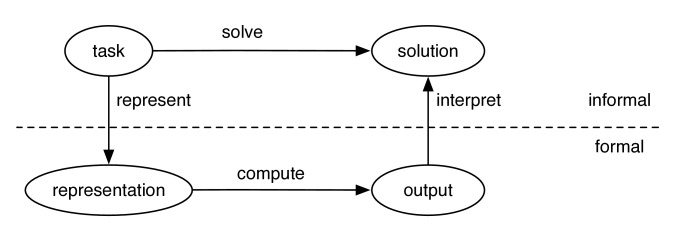
\includegraphics[scale=.65]{ruoloAgenti.png}
\end{center}
\end{figure}
Per risolvere un compito, il progettista di un sistema deve:
\begin{itemize}
\item determinare cosa costituisce una soluzione
\item rappresentare l'attività in un modo in cui un computer può ragionare
\item utilizzare il computer per calcolare un output, ovvero le risposte presentate a un utente o le azioni da eseguire nell'ambiente
\item interpretare l'output come una soluzione al compito.
\end{itemize}

\textbf{La conoscenza} è l'informazione su un dominio che può essere utilizzata per risolvere compiti in quel dominio. Per risolvere molti compiti è necessaria molta conoscenza e questa conoscenza deve essere rappresentata nel computer. Come parte della progettazione di un programma per risolvere compiti, dobbiamo definire come sarà rappresentata la conoscenza. Un \textbf{linguaggio di rappresentazione} viene utilizzato per esprimere la conoscenza utilizzata in un agente. \textbf{Una rappresentazione} di alcune conoscenze sono le particolari strutture di dati utilizzate per codificare la conoscenza in modo che possa essere ragionata. \textbf{Una base di conoscenza} è la rappresentazione di tutta la conoscenza memorizzata da un agente.
Un buon linguaggio di rappresentazione è un compromesso tra molti obiettivi concorrenti. Una rappresentazione dovrebbe essere:
\begin{itemize}
\item abbastanza ricco da esprimere le conoscenze necessarie per risolvere il compito
\item il più vicino possibile a una specificazione naturale del compito; dovrebbe essere compatto, naturale e manutenibile. Dovrebbe essere facile vedere la relazione tra la rappresentazione e il dominio rappresentato, in modo che sia facile determinare se la conoscenza rappresentata è corretta. Una piccola modifica nell'attività dovrebbe comportare una piccola modifica nella rappresentazione dell'attività
\item suscettibile di calcolo efficiente, o trattabile , il che significa che l'agente può agire abbastanza rapidamente. Per garantire ciò, le rappresentazioni sfruttano le caratteristiche dell'attività per il guadagno computazionale e compensano l'accuratezza e il tempo di calcolo
\item in grado di essere acquisito da persone, dati ed esperienze passate.
\end{itemize}

Data una descrizione informale di un'attività, prima ancora di considerare un computer, un progettista agente dovrebbe determinare cosa costituirebbe una soluzione. Questa domanda sorge non solo nell'IA, ma in qualsiasi progettazione di software. Gran parte dell'ingegneria del software implica il perfezionamento delle specifiche dell'attività. Le attività in genere non sono ben specificate. Non solo di solito c'è molto non specificato, ma anche le parti non specificate non possono essere compilate arbitrariamente. Data un'attività ben definita, il problema successivo è se è importante se la risposta restituita è errata o incompleta. Esistono quattro classi comuni di soluzioni:
\begin{itemize}
\item Una \textbf{soluzione ottimale} per un'attività è quella che è la soluzione migliore in base a una certa misura della qualità della soluzione.
\item Spesso un agente non ha bisogno della soluzione migliore per un'attività, ma ha solo bisogno di una soluzione. \textbf{Una soluzione soddisfacente} è quella che è abbastanza buona secondo una descrizione di quali soluzioni sono adeguate.
\item Uno dei vantaggi di una misura cardinale del successo è che consente approssimazioni. Una \textbf{soluzione approssimativamente ottimale} è quella la cui misura della qualità è vicina al meglio che potrebbe essere teoricamente ottenuto. In genere, gli agenti non necessitano di soluzioni ottimali per le attività; devono solo avvicinarsi abbastanza. Per alcune attività, dal punto di vista computazionale è molto più facile ottenere una soluzione approssimativamente ottimale che ottenere una soluzione ottimale. Tuttavia, per altre attività, è altrettanto difficile trovare una soluzione approssimativamente ottimale che sia garantita entro alcuni limiti dell'ottimo quanto trovare una soluzione ottimale.

\item \textbf{Una soluzione probabile} è quella che, anche se potrebbe non essere effettivamente una soluzione per l'attività, è probabile che sia una soluzione. Questo è un modo per approssimare, in modo preciso, una soluzione soddisfacente. Spesso si vuole distinguere il tasso di errore falso positivo (la proporzione di risposte fornite dal computer che non sono corrette) dal tasso di errore falso negativo (la proporzione di quelle risposte non fornite dal computer che sono effettivamente corrette). Alcune applicazioni sono molto più tolleranti di uno di questi tipi di errori rispetto all'altro.
\end{itemize}

Una volta che hai alcuni requisiti sulla natura di \textbf{una soluzione}, devi rappresentare l'attività in modo che un computer possa risolverla. I computer e le menti umane sono esempi di sistemi di simboli fisici. \textbf{Un simbolo} è un modello significativo che può essere manipolato. Esempi di simboli sono parole scritte, frasi, gesti, segni su carta o sequenze di bit. Un sistema di simboli crea, copia, modifica e distrugge i simboli. In sostanza, un simbolo è uno dei modelli manipolati come unità da un sistema di simboli. Viene usato il termine fisico, perché i simboli in un sistema di simboli fisici sono oggetti fisici che fanno parte del mondo reale, anche se possono essere interni ai computer e al cervello. Potrebbero anche aver bisogno di influenzare fisicamente l'azione o il controllo motorio. Gran parte dell'IA si basa sull'ipotesi del sistema di simboli fisici di Newell e Simon: Un sistema di simboli fisici ha i mezzi necessari e sufficienti per un'azione intelligente generale.

Significa che qualsiasi agente intelligente è necessariamente un sistema di simboli fisici. Significa anche che un sistema di simboli fisici è tutto ciò che è necessario per un'azione intelligente; non è richiesta alcuna magia o un fenomeno quantistico ancora da scoprire. Non implica che un sistema di simboli fisici non abbia bisogno di un corpo per percepire e agire nel mondo. Si discute se le variabili nascoste, a cui non è stato assegnato un significato, ma sono utili, possano essere considerate come simboli. L'ipotesi del sistema dei simboli fisici è un'ipotesi empirica che, come altre ipotesi scientifiche, deve essere giudicata da quanto bene si adatta alle prove e da quali ipotesi alternative esistono. In effetti, potrebbe essere falso.

Un agente intelligente può essere visto come un manipolatore di simboli per produrre azioni. Molti di questi simboli sono usati per riferirsi a cose nel mondo. Altri simboli possono essere concetti utili che possono avere o meno un significato esterno. Ancora altri simboli possono riferirsi a stati interni dell'agente. Un agente può utilizzare un sistema di simboli fisici per modellare il mondo. \textbf{Un modello} di mondo è una rappresentazione delle convinzioni di un agente su ciò che è vero nel mondo o su come il mondo cambia. Il mondo non deve essere modellato al livello più dettagliato per essere utile. Tutti \textbf{i modelli} sono astrazioni ; rappresentano solo una parte del mondo e tralasciano molti dettagli. Un agente può avere un modello molto semplicistico del mondo, oppure può avere un modello molto dettagliato del mondo. \textbf{Il livello di astrazione} fornisce un ordinamento parziale dell'astrazione. Un'astrazione di livello inferiore include più dettagli rispetto a un'astrazione di livello superiore. Un agente può avere modelli del mondo multipli, anche contraddittori. I modelli vengono giudicati non in base alla loro correttezza, ma in base alla loro utilità.

La scelta di un livello di astrazione appropriato è difficile per i seguenti motivi:
\begin{itemize}
\item Una descrizione di alto livello è più facile da specificare e comprendere per un essere umano.
\item Una descrizione di basso livello può essere più accurata e più predittiva. Spesso le descrizioni di alto livello sottraggono dettagli che possono essere importanti per risolvere effettivamente il compito.
\item Più basso è il livello, più difficile è ragionare. Questo perché una soluzione a un livello di dettaglio inferiore comporta più passaggi ed esistono molte più possibili linee di azione tra cui scegliere.
\item Un agente potrebbe non conoscere le informazioni necessarie per una descrizione di basso livello.
\end{itemize}

Spesso è una buona idea modellare un ambiente a più livelli di astrazione. Due tipi di livelli di astrazione molto comuni sono:
\begin{itemize}
\item \textbf{Il livello di conoscenza} è il livello di astrazione che considera ciò che un agente conosce e crede e quali sono i suoi obiettivi. Il livello di conoscenza considera ciò che un agente sa, ma non come ragiona. Ad esempio, il comportamento dell'addetto alle consegne può essere descritto in base al fatto che sappia che un pacco è arrivato o meno e se sa dove si trova o meno una determinata persona. Sia gli agenti umani che quelli robotici sono descrivibili a livello di conoscenza. A questo livello, non si specifica come verrà calcolata la soluzione e nemmeno quale delle tante possibili strategie a disposizione dell'agente verrà utilizzata.
\item \textbf{Il livello del simbolo} è un livello di descrizione di un agente in termini di ragionamento che fa. Per implementare il livello di conoscenza, un agente manipola i simboli per produrre risposte. Molti esperimenti di scienze cognitive sono progettati per determinare quale manipolazione dei simboli avviene durante il ragionamento. Mentre il livello di conoscenza riguarda ciò che l'agente crede del mondo esterno e quali sono i suoi obiettivi in termini di mondo esterno, il livello simbolico riguarda ciò che accade all'interno di un agente per ragionare sul mondo esterno.
\end{itemize}

\subsubsection{Spazio di progettazione dell'agente}

Gli agenti che agiscono in ambienti variano in complessità, dai termostati alle aziende con obiettivi multipli che agiscono in ambienti competitivi. Qui descriviamo dieci dimensioni di complessità nella progettazione di agenti intelligenti. Queste dimensioni possono essere considerate separatamente ma devono essere combinate per creare un agente intelligente. Queste dimensioni definiscono uno spazio di progettazione per l'IA; punti diversi in questo spazio si ottengono variando i valori su ciascuna dimensione. Queste dimensioni danno una divisione grossolana dello spazio di progettazione per gli agenti intelligenti. Ci sono molte altre scelte progettuali che devono essere fatte anche per costruire un agente intelligente.

La prima dimensione è il livello di \textbf{modularità}. La modularità è la misura in cui un sistema può essere scomposto in moduli interagenti che possono essere compresi separatamente. La modularità è importante per ridurre la complessità. È evidente nella struttura del cervello, serve come base per l'informatica ed è un aspetto importante di qualsiasi grande organizzazione. La modularità è tipicamente espressa in termini di scomposizione gerarchica. Nella dimensione della modularità , la struttura di un agente è una delle seguenti:
\begin{itemize}
\item \textbf{piatta}: non esiste una struttura organizzativa
\item \textbf{modulare}: il sistema è scomposto in moduli integrati che posono essere compresi da soli
\item \textbf{gerarchico}: il sistema è modulare e i moduli stessi sono scomposti in moduli più semplici, ciascuno dei quali è un sistema gerarchico o semplici componenti.
\end{itemize}

In una struttura piatta o modulare l'agente ragiona tipicamente a un unico livello di astrazione. In una struttura gerarchica l'agente ragiona a più livelli di astrazione. I livelli inferiori della gerarchia implicano il ragionamento a un livello inferiore di astrazione. Una scomposizione gerarchica è importante per ridurre la complessità della creazione di un agente intelligente che agisce in un ambiente complesso. L'astrazione procedurale e la programmazione orientata agli oggetti in informatica sono progettate per consentire la semplificazione di un sistema sfruttando la modularità e l'astrazione. Per esplorare le altre dimensioni, inizialmente ignoriamo la struttura gerarchica e assumiamo una rappresentazione piatta. Ignorare la scomposizione gerarchica spesso va bene per attività di piccole o medie dimensioni, come per animali semplici, piccole organizzazioni o programmi per computer di dimensioni piccole o moderate. Quando le attività dei sistemi diventano complessi, è necessaria un'organizzazione gerarchica.

La dimensione dell'orizzonte di pianificazione indica quanto avanti nel tempo l'agente pianifica. Fino a che punto l'agente "guarda al futuro" quando decide cosa fare è chiamato \textbf{orizzonte di pianificazione}. Per completezza, includiamo il caso di non pianificazione in cui l'agente non sta ragionando in tempo. I punti temporali considerati da un agente durante la pianificazione sono chiamati fasi. Nella dimensione dell'orizzonte di pianificazione , un agente è uno dei seguenti:
\begin{itemize}
\item un \textbf{agente non pianificatore} è un agente che non considera il futuro quando decide cosa fare o quando il tempo non è coinvolto
\item un pianificatore di \textbf{orizzonte finito} è un agente che cerca un numero finito fisso di fasi
\item un pianificatore di \textbf{orizzonte indefinito} è un agente che guarda avanti un numero finito, ma non predeterminato, di fasi.
\item un pianificatore di \textbf{orizzonte infinito} è un agente che prevede di andare avanti per sempre. Questo è spesso chiamato processo
\end{itemize}

La \textbf{dimensione della rappresentazione} riguarda il modo in cui viene descritto il mondo.I diversi modi in cui il mondo potrebbe essere sono chiamati stati . Uno stato del mondo specifica lo stato interno dell'agente (il suo stato di credenza) e lo stato ambientale. Al livello più semplice, un agente può ragionare esplicitamente in termini di stati identificati individualmente. Invece di enumerare gli stati, è spesso più facile ragionare in termini di caratteristiche dello stato o di proposizioni vere o false dello stato. Uno stato può essere descritto in termini di caratteristiche , dove una caratteristica ha un valore in ogni stato. Una proposizione è una caratteristica booleana, il che significa che il suo valore è true o false. Quando si descrive un mondo complesso, le caratteristiche possono dipendere da relazioni e individui . Ciò che chiamiamo individuo potrebbe anche essere chiamato cosa , oggetto o entità . Una relazione su un singolo individuo è una proprietà . C'è una caratteristica per ogni possibile relazione tra gli individui. Ragionando in termini di relazioni e individui, un agente può ragionare su intere classi di individui senza mai enumerare le caratteristiche o le proposizioni, per non parlare degli stati. Un agente può dover ragionare su insiemi infiniti di individui, come l'insieme di tutti i numeri o l'insieme di tutte le frasi. Per ragionare su un numero illimitato o infinito di individui, un agente non può ragionare in termini di stati o caratteristiche; deve ragionare a livello relazionale. Nella \textbf{dimensione della rappresentazione}, l'agente ragiona in termini di:
\begin{itemize}
\item stati
\item caratteristiche
\item individui e relazioni
\end{itemize}

A volte un agente può decidere la sua azione migliore abbastanza rapidamente da poter agire. Spesso ci sono limiti di risorse computazionali che impediscono a un agente di eseguire l'azione migliore. Cioè, l'agente potrebbe non essere in grado di trovare l'azione migliore abbastanza rapidamente entro i suoi limiti di memoria per agire mentre quell'azione è ancora la cosa migliore da fare. Spesso, invece, un agente deve scambiare quanto tempo impiega per ottenere una soluzione con quanto è buona la soluzione; potrebbe essere meglio trovare rapidamente una soluzione ragionevole piuttosto che trovare una soluzione migliore in seguito perché il mondo sarà cambiato durante il calcolo.
\end{document}





